\section{Simulation}
\label{ch:simulation}

The simulations of the controller will be performed using Matlab and Simulink, simulating a model of the Aerosonde UAV. 

\begin{figure}[]
    \centering
    \makebox[\textwidth][c]{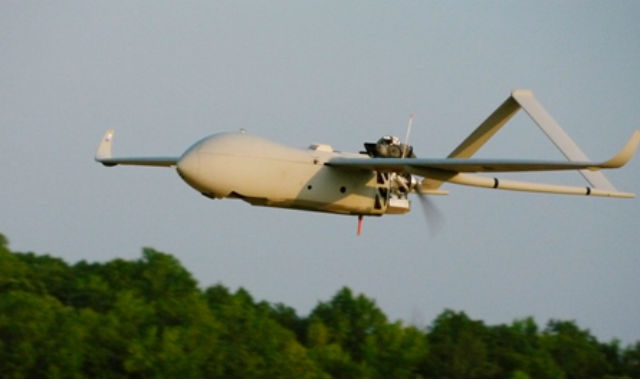
\includegraphics[width=0.9\textwidth, keepaspectratio=true]{aerosonde_image.jpg}}
    \caption{The Aerosonde UAV \cite{image}.}
	\label{fig:aerosonde}
\end{figure}

\subsection{Model}

The model of the Aerosonde UAV is based on parameters and equations given by Beard \& McLain \cite{suaBEARD}. The model was implemented by Gryte as a part of his master thesis \cite{GRYTE}.

The model is split into two parts, forces and aircraft dynamics. The forces module implements the equations for describing all the forces working on the aircraft, based on wind, aircraft states and the control inputs. The calculated forces are then sent to the aircraft dynamics module which calculates the new states of the aircraft based on the forces.


\subsection{Autopilot}

The autopilot used in the simulations has also been implemented by Gryte \cite{GRYTE}, and it is based on equations in Beard \& McLain \cite{suaBEARD} as well. The autopilot have previously been used with a different UAV, and therefore the controller gains needed to be tuned in order to control the Aerosonde UAV. The controller loops are defined by relative damping factor $\zeta$ and natural frequency $\omega_n$, and by implementing the control loops outside the model the parameters can be found separately. This makes a good starting point for further tuning.

\subsection{Path Follower}
\label{ch:path_follower}

Three different path followers will be used in this simulation. One of the three path followers will be used to navigate between waypoints by the rudder controller, while the other two will be used to follow the paths generated by the path planner.

The strategy used to follow Dubins path will be based on two algorithms presented by Beard \& McLain \cite{suaBEARD}. The two algorithms are used to follow straight and curved line paths.

In order to follow straight line paths, the algorithm uses the position and course of the aircraft, the previous waypoint and the direction from the previous to the next waypoint as input. The previous waypoint and the direction to the next waypoint are given as output from the algorithm generating Dubins path described in chapter \ref{ch:dubins_path}. The new course is calculated so that the aircrafts position will converge towards the original path.

The algorithm for following circular paths is based on following perfect circles. Therefore it takes center and radius of the circle, the direction to orbit the circle, and the current position and course of the aircraft. The desired course calculated here will also ensure that the aircrafts position converges to the circular path.

The altered path is based on the actual position of the UAV when following the Dubins path in the first simulation, and will therefore not consist of circular arcs and straight lines. Instead the path will be a continuous path which requires a different path follower. The path follower will be based on the principles of Line Of Sight (LOS) steering laws presented by Fossen \cite{fartoyFOSSEN}.

Enclosure-based steering is a LOS principle that considers a circle with radius $R$ enclosing the vehicle, which represents the LOS distance, shown in figure \ref{fig:path_los}. Assuming that the radius is sufficiently large compared to the vehicle's distance from the path, the circle will intersect the path at two different points. One of the points will be in the direction of the vehicle, denoted $x_{los}$ and $y_{los}$. This is the point the vehicle will be directed to, and the course to that point can be expressed as \cite{fartoyFOSSEN}:

\begin{equation}
	\chi_d(t) = \text{atan2}(y_{los} - y(t), x_{los} - x(t))
\end{equation}

where $x(t)$ and $y(t)$ is the vehicle's current position. Using Pythagoras theorem, the points $x_{los}$ and $y_{los}$ can be found as:

\begin{equation}
	[x_{los} - x(t)]^2 + [y_{los} - y(t)]^2 = R^2
\end{equation}

where $R$ is the chosen LOS distance.

\begin{figure}
	\import{/}{path_los.tex}
	\caption{Illustration of enclosed line-of-sight path following.}
	\label{fig:path_los}
\end{figure}

The last path follower used to navigate between waypoints is also based on an algorithm by Beard \& McLain \cite{suaBEARD}, and is a simpler algorithm than the one for Dubins path. It calculates the unit vectors between the waypoints and uses these to detect when the aircraft passes a waypoint. The algorithm returns the last waypoint visited and the direction for the next waypoint, which can be passed along to the algorithm to follow straight line paths already described. This will be used when simulating the controller in chapter \ref{ch:controller_sim}.